\section{Tecnologie NoSQL: Sistemi Document-Based}

\begin{figure}[H]
    \centering
    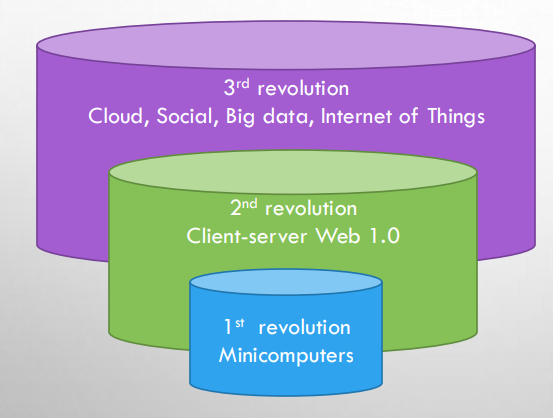
\includegraphics[width=0.75\linewidth]{image52.png}
    \caption{Evoluzione Database}
\end{figure}

La figura mostra l'evoluzione storica delle tecnologie di database attraverso
tre grandi rivoluzioni, rappresentate come livelli sovrapposti. Ogni rivoluzione
introduce nuovi modelli, nuovi paradigmi e nuove esigenze dovute ai cambiamenti
tecnologici del periodo.

\subsection*{Prima rivoluzione (1950--1960)}
Alla base si trova la prima rivoluzione dei database, nata nell'epoca dei
\textbf{minicomputer}. In questo periodo emergono i primi sistemi per la gestione
dei dati, caratterizzati da strutture rigide e fortemente dipendenti
dall'organizzazione fisica dei file. Le principali tecnologie di questo periodo sono:
\begin{itemize}
    \item database \textbf{gerarchici};
    \item database \textbf{reticolari} (network databases);
    \item file organizzati tramite \textbf{ISAM} (Indexed Sequential Access Method).
\end{itemize}

\subsection*{Seconda rivoluzione (1970--1990)}
Il secondo livello corrisponde alla diffusione del modello \textbf{relazionale},
che nasce negli anni '70 grazie ai lavori di E. F. Codd. In questa fase il
paradigma relazionale si impone come standard grazie alla sua semplicità,
astrazione e indipendenza dalla struttura fisica dei dati.
È l'epoca dei sistemi \textbf{client-server} e del Web~1.0.

\subsection*{Terza rivoluzione (2005--oggi)}
La terza rivoluzione si sviluppa nell'era del \textbf{cloud}, dei \textbf{big data}
e dell'\textbf{Internet of Things}. In questo contesto il volume, la varietà e la
velocità dei dati aumentano notevolmente, rendendo necessarie nuove soluzioni
oltre al modello relazionale classico. Accanto ai database tradizionali si
diffondono:
\begin{itemize}
    \item sistemi \textbf{NoSQL};
    \item sistemi \textbf{NewSQL};
    \item piattaforme di \textbf{Big Data}.
\end{itemize}

Questa rivoluzione rappresenta un ampliamento, non una sostituzione: i database
relazionali restano fondamentali, ma vengono affiancati da tecnologie progettate
per gestire grandi moli di dati distribuiti.

\subsection{Approcci NoSQL}
I modelli NoSQL nascono per rispondere ai limiti dei tradizionali database
relazionali in scenari caratterizzati da grandi quantità di dati, alta
eterogeneità e necessità di scalare orizzontalmente. Questi sistemi adottano
strutture più flessibili e meno vincolate rispetto allo schema rigido delle
tabelle relazionali, permettendo una gestione più efficiente di dati distribuiti
su larga scala. Tra gli approcci più diffusi troviamo:
\begin{itemize}
    \item \textbf{Sistemi Key-Value}: tutti i dati sono rappresentati tramite coppie
    (chiave, valore), dove la chiave identifica le istanze e il valore può avere
    una qualsiasi struttura, anche non omogenea. Un esempio di questo approccio
    è Hadoop.

    \item \textbf{Sistemi Document-Store}: i dati sono rappresentati come collezioni
    di documenti con struttura complessa e senza schema fisso.
    Esempi: \textbf{MongoDB}, \textbf{CouchBase}.

    \item \textbf{Column Store}: i dati sono rappresentati tramite record con struttura variabile.
    Esempi: \textbf{BigTable}, \textbf{HBase}, \textbf{Cassandra}.

    \item \textbf{Graph-Store}: i dati sono rappresentati come grafi, con nodi e archi.
    Esempi: \textbf{Neo4j}, \textbf{OrientDB}.
\end{itemize}

\subsection{Sistemi Document-Store}
Caratteristiche principali:
\begin{itemize}
    \item i dati sono organizzati come collezioni di \textbf{documenti};
    \item ogni documento può contenere dati complessi e nidificati;
    \item l'\textbf{incapsulamento} è fondamentale: tutte le informazioni relative a un'entità
    stanno nello stesso documento;
    \item non è richiesto uno schema fisso: i documenti di una collezione possono avere
    strutture diverse.
\end{itemize}

\subsubsection*{Progettazione dei dati come documenti}
Decisioni fondamentali:
\begin{itemize}
    \item scelta della chiave di accesso;
    \item struttura interna dei documenti e livello di incapsulamento;
    \item rappresentazione delle relazioni tra documenti.
\end{itemize}

Le relazioni possono essere modellate tramite:
\begin{itemize}
    \item \textbf{riferimenti} (ID dell’altro documento);
    \item \textbf{documenti nidificati}.
\end{itemize}

\begin{figure}[H]
    \centering
    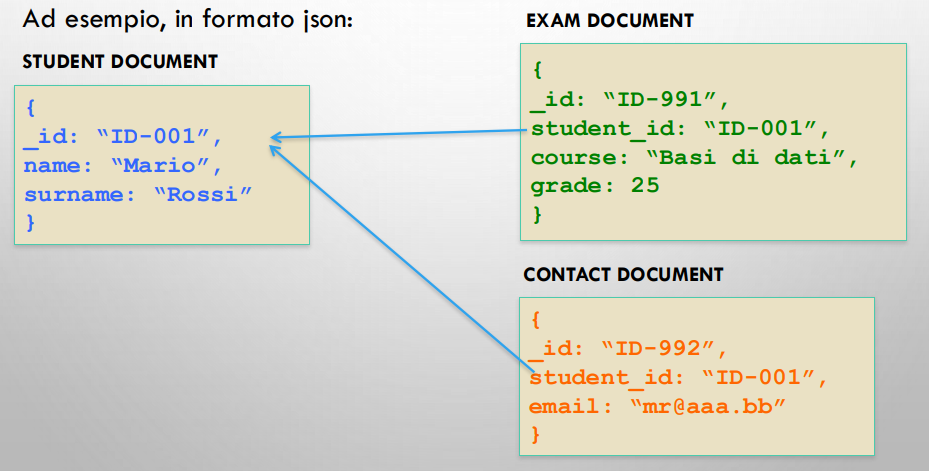
\includegraphics[width=0.75\linewidth]{image53.png}
    \caption{Formato JSON}
\end{figure}

\subsection{Regole di traduzione di uno schema ER in collezioni di documenti}

Assunzioni preliminari:
\begin{itemize}
    \item si adotta un approccio \textbf{embedded};
    \item lo schema ER è privo di generalizzazioni;
    \item relazioni ternarie o superiori eliminate;
    \item identificate collezioni \(\{DOC_1, ..., DOC_N\}\).
\end{itemize}

\subsubsection*{Regole fondamentali}
\begin{enumerate}
    \item Ogni collezione \(DOC_i\) corrisponde a un'entità principale.
    \item Ogni istanza dell'entità principale produce un documento.
    \item Le entità non principali vengono incapsulate nella principale.
    \item Le relazioni sono rappresentate tramite incapsulamento o riferimenti.
\end{enumerate}

\subsubsection{Prima Fase (entità principali)}
\begin{figure}[H]
    \centering
    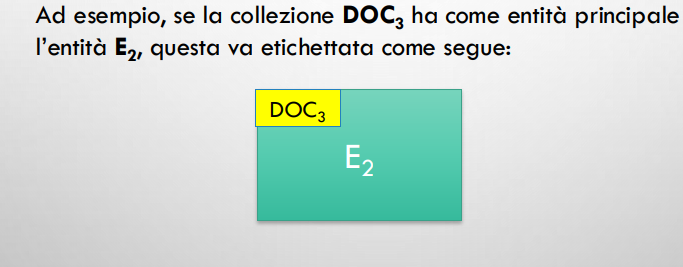
\includegraphics[width=1\linewidth]{image56.png}
    \caption{Individuazione entità principali}
\end{figure}

\subsubsection{Seconda Fase (incapsulamento entità non principali)}
\begin{figure}[H]
    \centering
    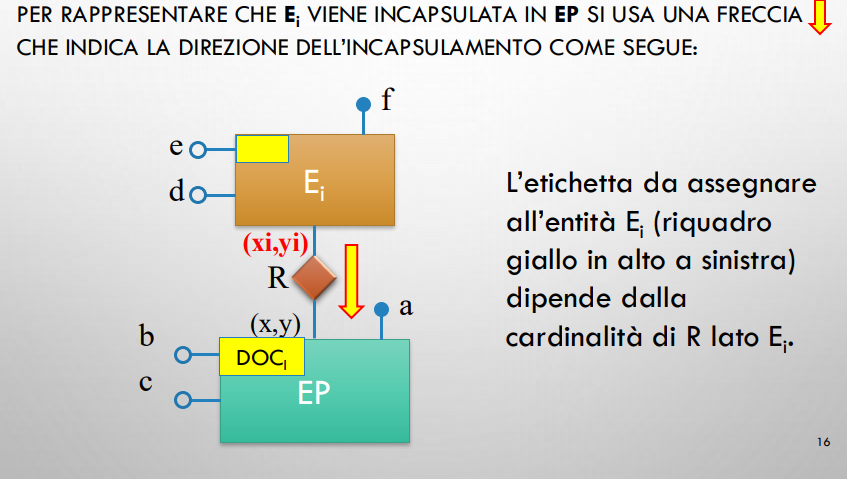
\includegraphics[width=0.75\linewidth]{image57.png}
    \caption{Incapsulamento}
\end{figure}

\subsection*{Diversi Casi}
\begin{figure}[H]
    \centering
    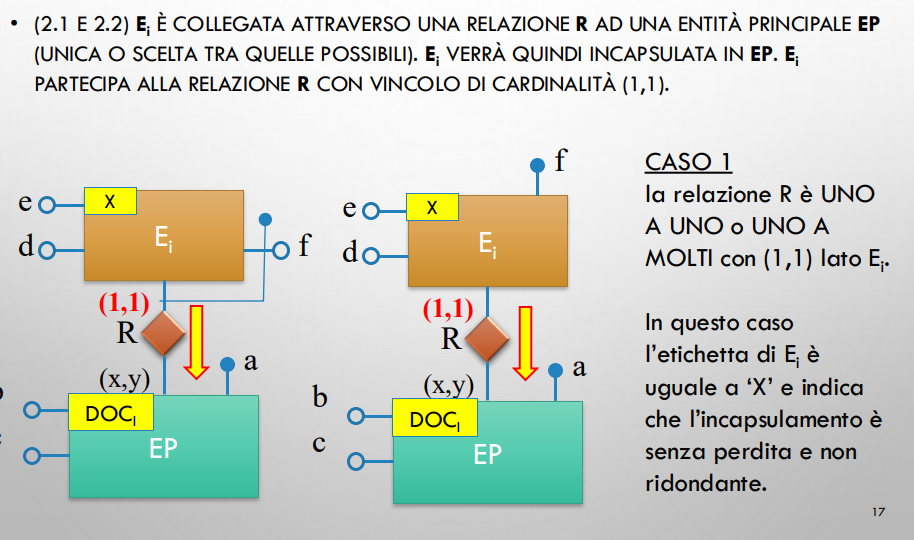
\includegraphics[width=1\linewidth]{image58.png}
    \caption{Uno a uno o uno a molti con (1,1)}
\end{figure}

\begin{figure}[H]
    \centering
    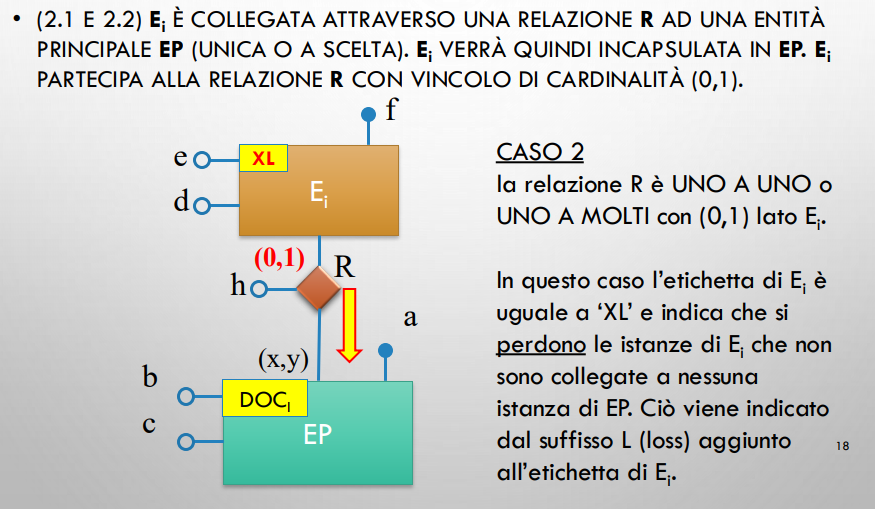
\includegraphics[width=1\linewidth]{image59.png}
    \caption{Uno a uno o uno a molti con (0,1)}
\end{figure}

\begin{figure}[H]
    \centering
    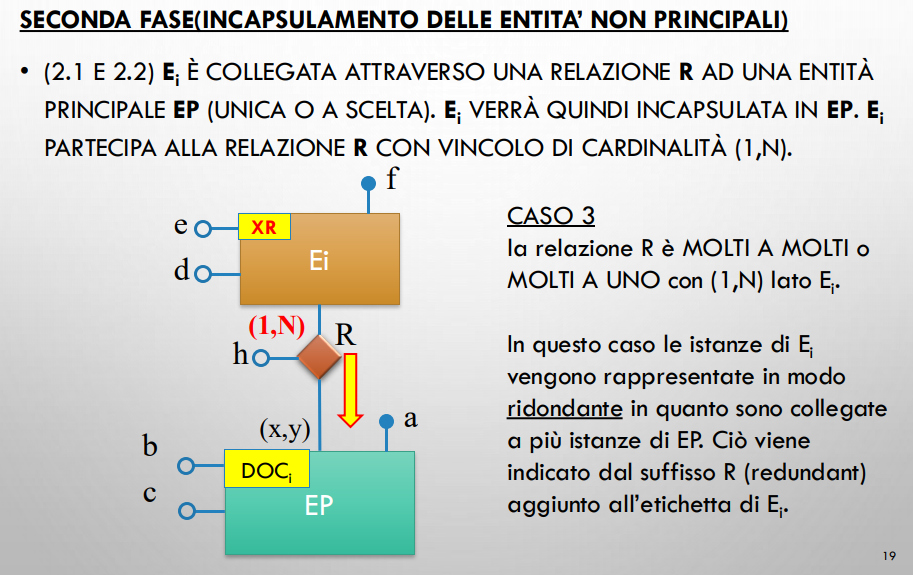
\includegraphics[width=1\linewidth]{image60.png}
    \caption{Molti a molti o molti a uno con (1,N)}
\end{figure}

\begin{figure}[H]
    \centering
    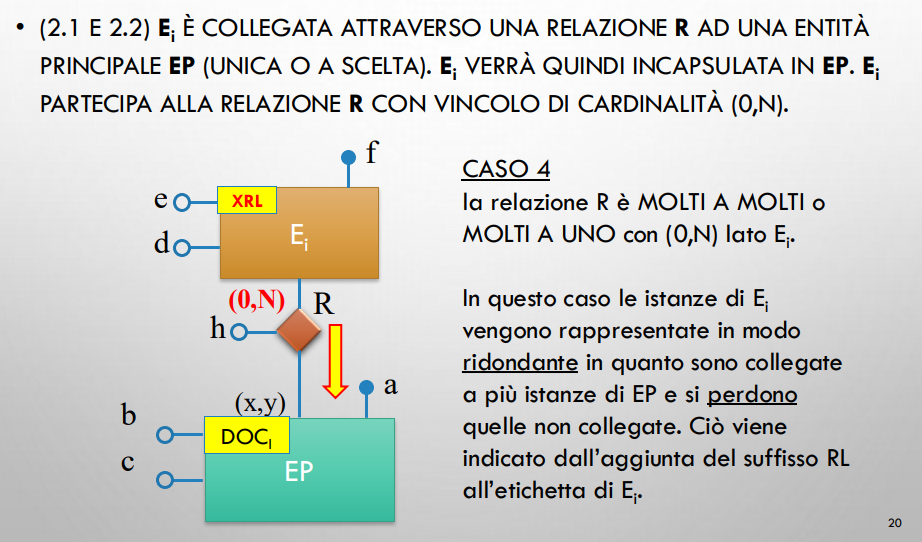
\includegraphics[width=1\linewidth]{image61.png}
    \caption{Molti a molti o molti a uno con (0,N) lato Ei}
\end{figure}

\subsubsection{Terza Fase (relazioni non strutturali)}
\begin{figure}[H]
    \centering
    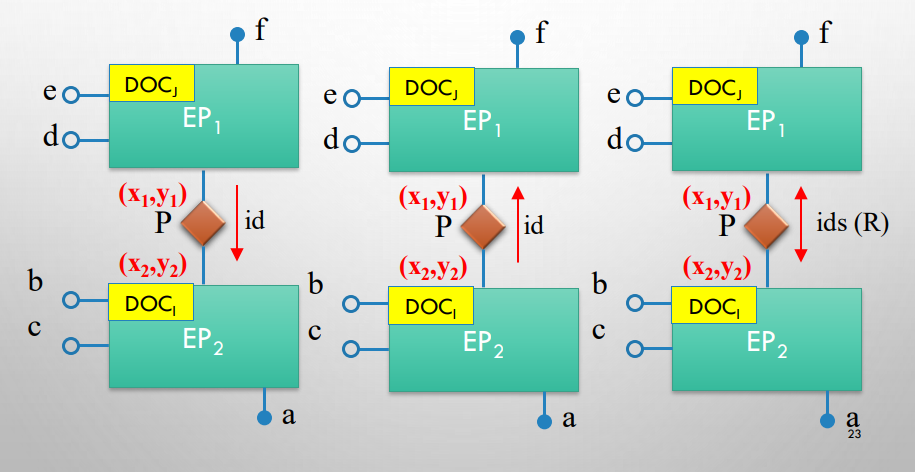
\includegraphics[width=1\linewidth]{image63.png}
    \caption{Etichettatura dello schema ER}
\end{figure}

\subsubsection*{Casi particolari}
\begin{figure}[H]
    \centering
    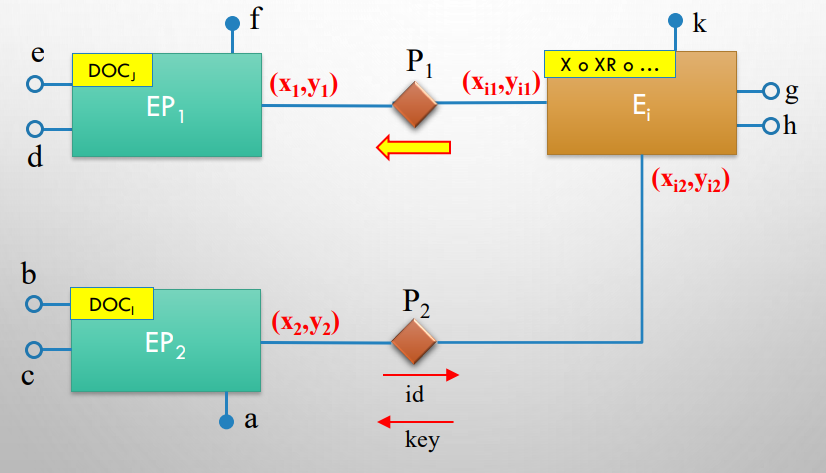
\includegraphics[width=1\linewidth]{image64.png}
    \caption{Caso Particolare A}
\end{figure}

\begin{figure}[H]
    \centering
    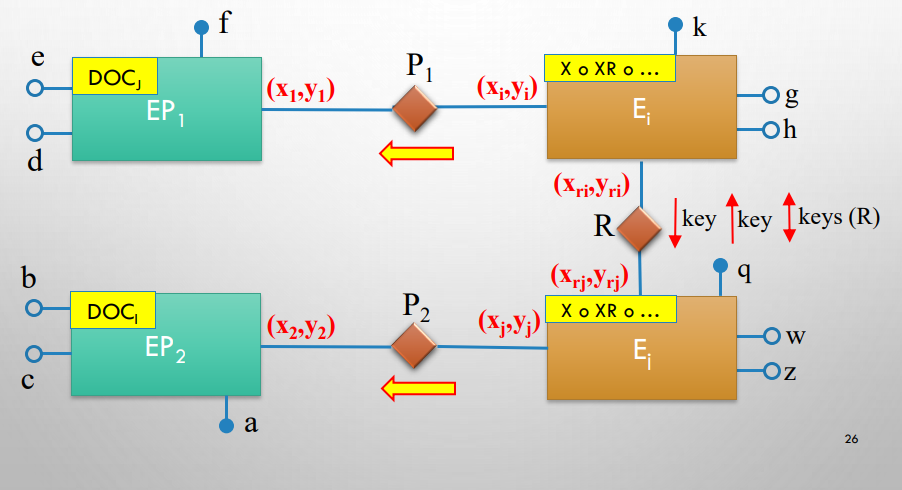
\includegraphics[width=1\linewidth]{image65.png}
    \caption{Caso Particolare B}
\end{figure}

\subsection{Quarta fase}
\begin{figure}[H]
    \centering
    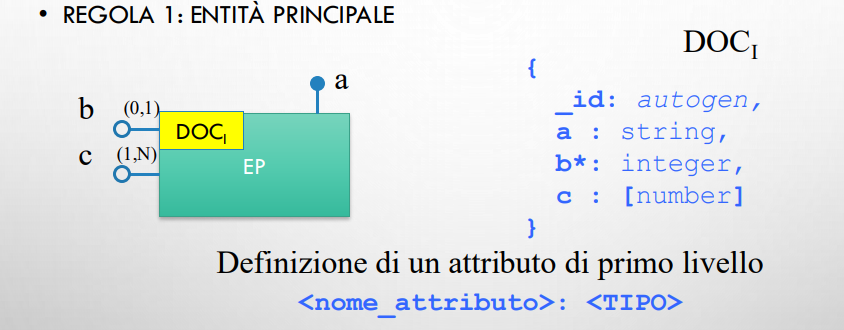
\includegraphics[width=1\linewidth]{image66.png}
    \caption{Entità Principale}
\end{figure}

\texttt{<TIPO>} può essere: string, integer, number, boolean, date, time, timestamp.

L'attributo \texttt{\_id} è sempre autogenerato dal sistema.

\begin{figure}[H]
\centering
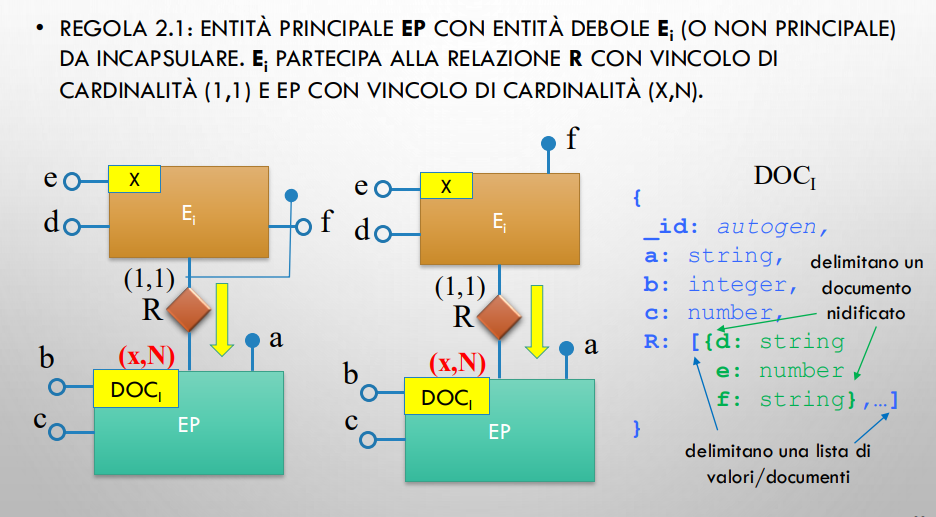
\includegraphics[width=1\linewidth]{image67.png}
\end{figure}

\begin{figure}[H]
\centering
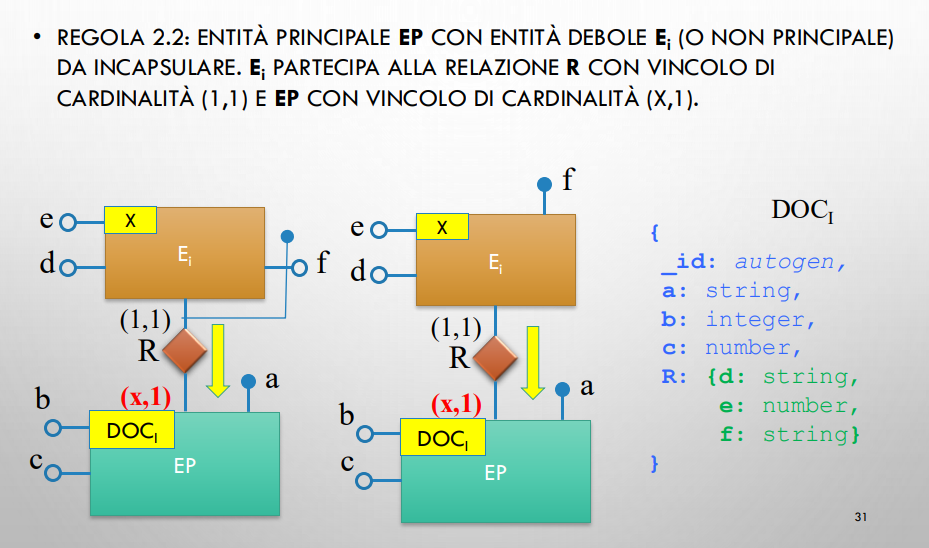
\includegraphics[width=1\linewidth]{image68.png}
\end{figure}

\begin{figure}[H]
\centering
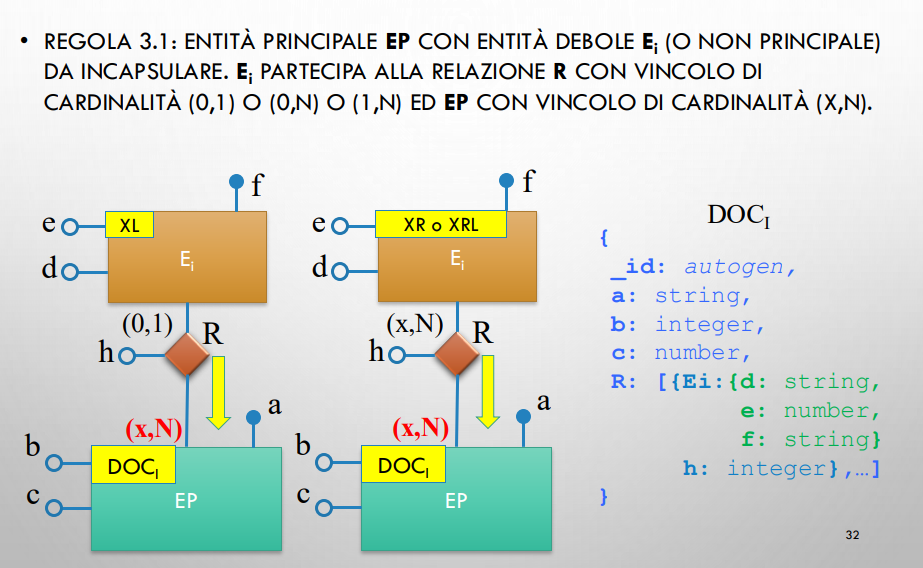
\includegraphics[width=1\linewidth]{image69.png}
\end{figure}

\begin{figure}[H]
\centering
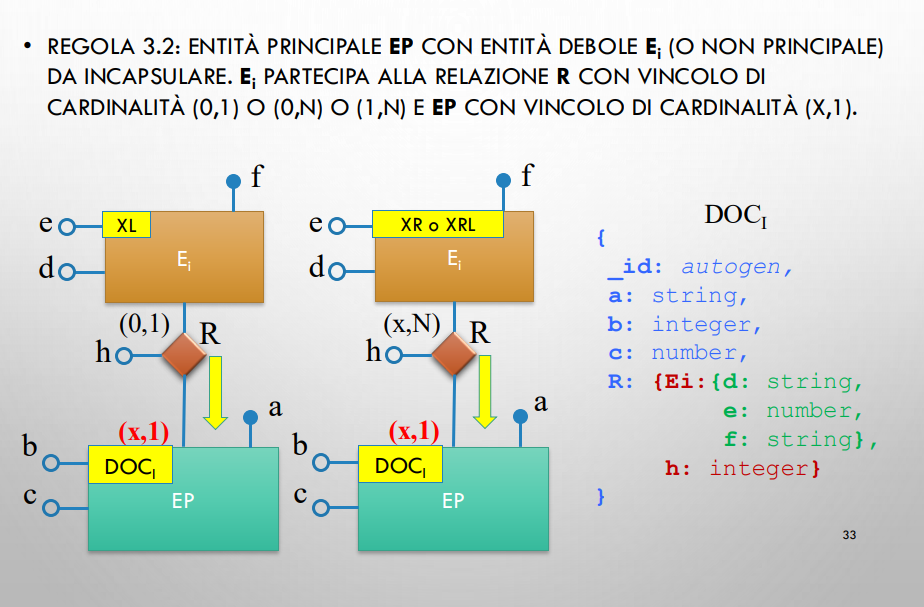
\includegraphics[width=1\linewidth]{image70.png}
\end{figure}

\begin{figure}[H]
\centering
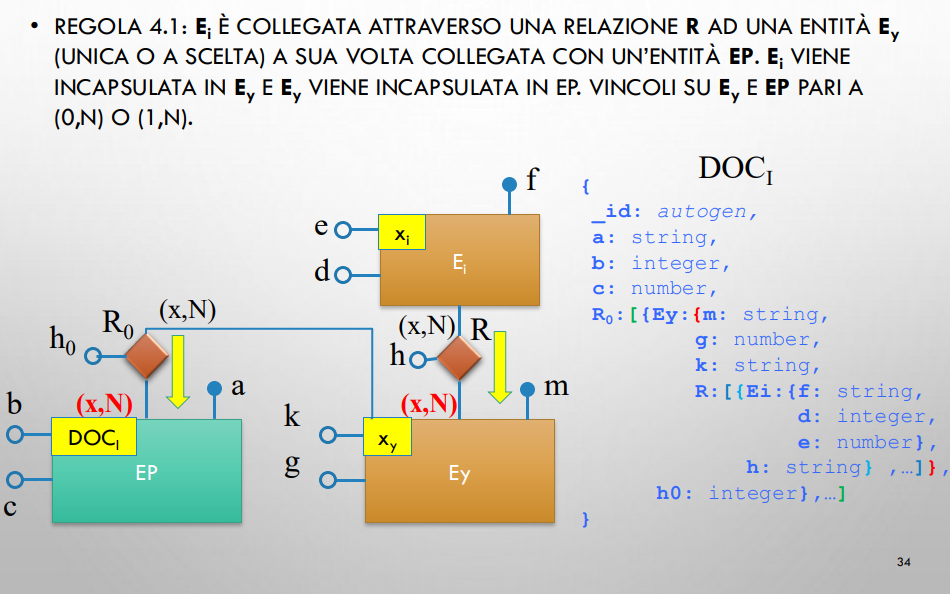
\includegraphics[width=1\linewidth]{image71.png}
\end{figure}

\begin{figure}[H]
\centering
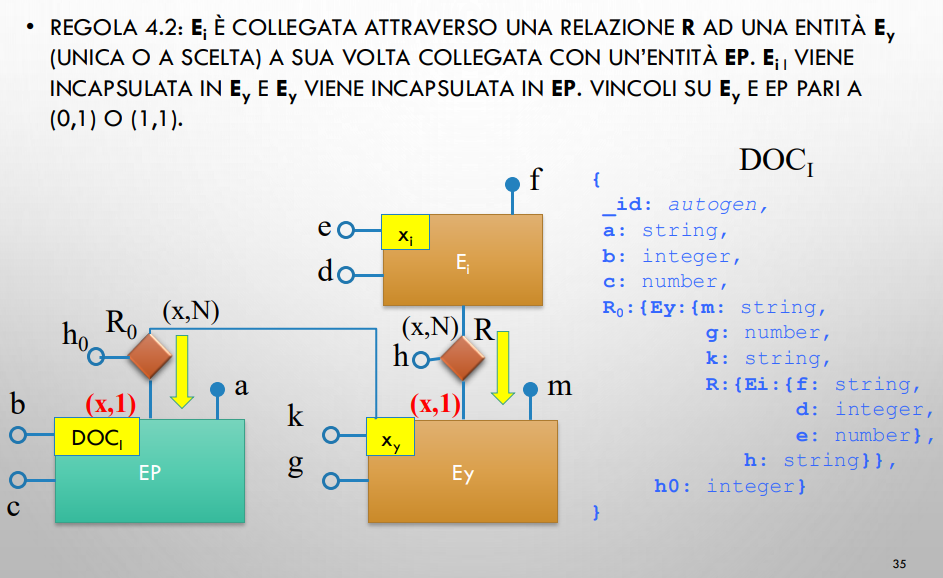
\includegraphics[width=1\linewidth]{image72.png}
\end{figure}

\begin{figure}[H]
\centering
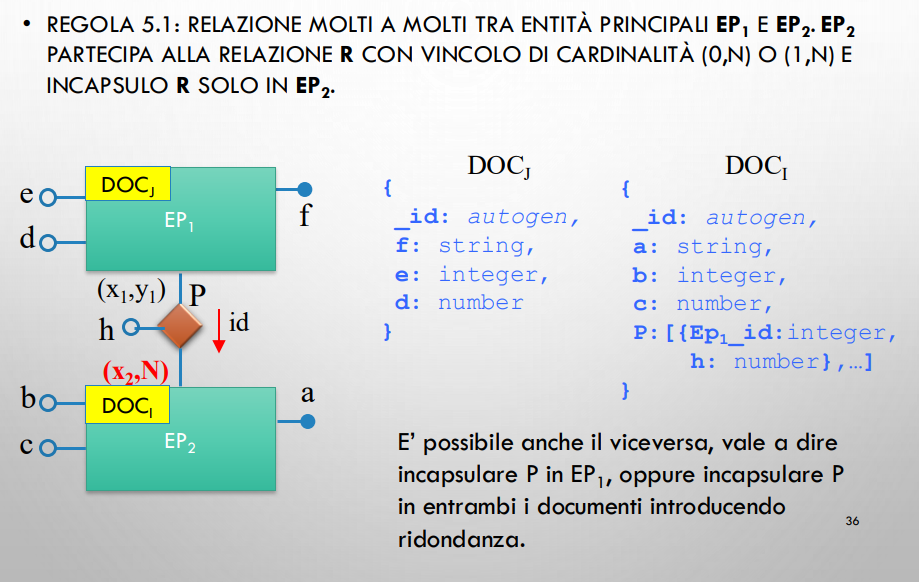
\includegraphics[width=1\linewidth]{image73.png}
\end{figure}

\begin{figure}[H]
\centering
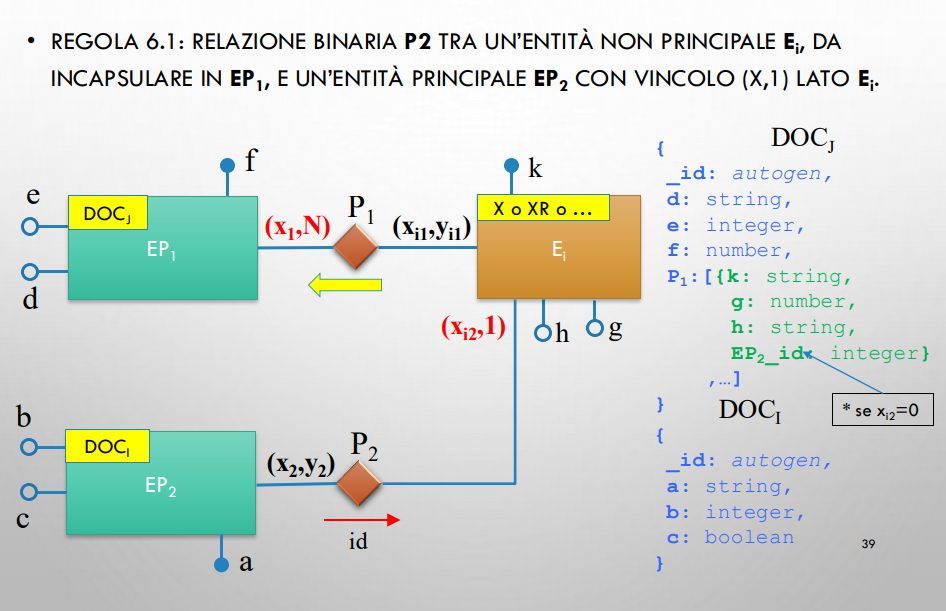
\includegraphics[width=1\linewidth]{image74.png}
\end{figure}

\begin{figure}[H]
\centering
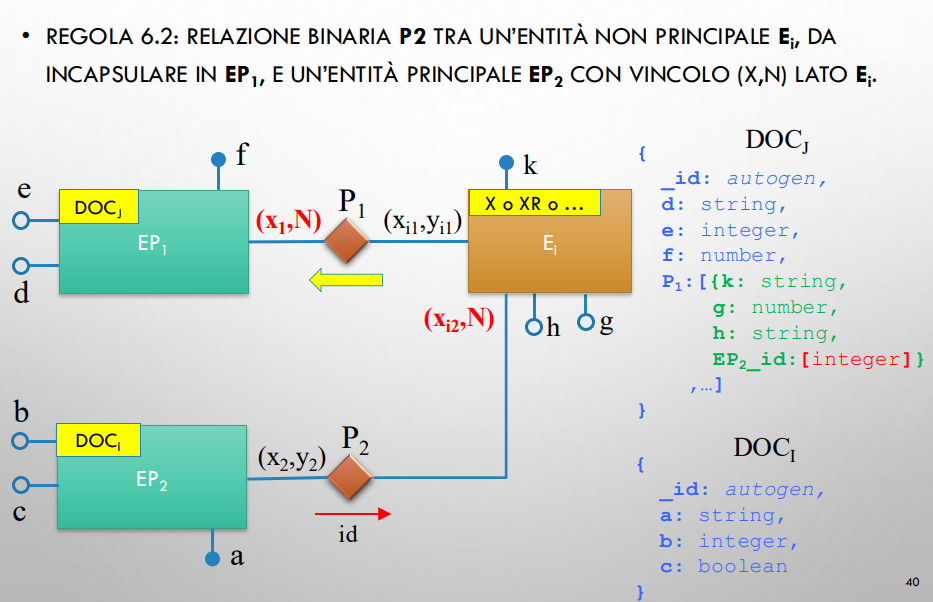
\includegraphics[width=1\linewidth]{image75.png}
\end{figure}

\begin{figure}[H]
\centering
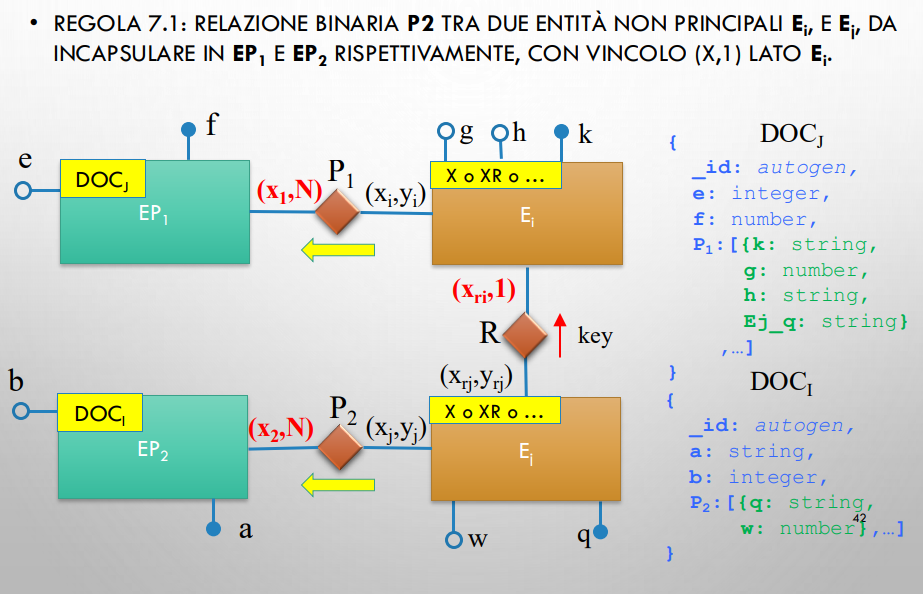
\includegraphics[width=1\linewidth]{image76.png}
\end{figure}

\begin{figure}[H]
\centering
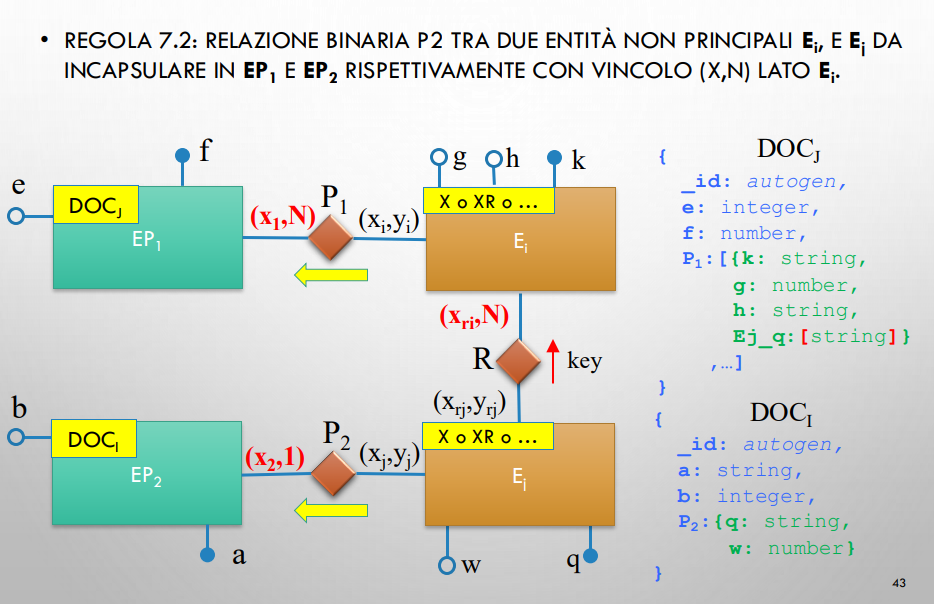
\includegraphics[width=1\linewidth]{image77.png}
\end{figure}
